\section{实验过程}

该部分主要呈现实验的具体流程,介绍实验使用的基本方法与基本工具,并且阐明个中细节,展示主要解决的几个问题。

\subsection{训练数据提取与处理}

\begin{figure}[ht]
	\centering
	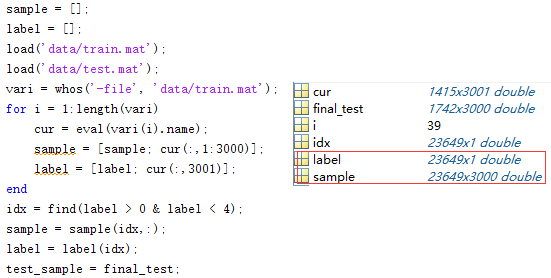
\includegraphics[width=.8\linewidth]{readin}
	\caption{读入数据}
	\label{fig:readin}
\end{figure}

首先将39个人的所有数据合并,然后过滤掉第四和第五周期的数据。继而将标签与特征数据分离,易于后期进行训练。

最终将数据分成两部分,一部分是训练特征,另一部分是标签。此外还有一个最终测试样本,但是不包含标签。

\subsubsection{三类训练样本的比例对比}

为了更直观的呈现新给的样本集合中每一类样本所占有的比例,以明确后续训练过程中的细节,
我组尝试将三类样本占总样本的比例算出,可知,第一类样本占有11.68\%,
第二类占有74.2\%,第三类占有14.00\%,由于第二类样本较多,另外两类的样本显然较少,
这也是我组在进行后续优化所要考虑的问题。

\begin{figure}[ht]
	\centering
	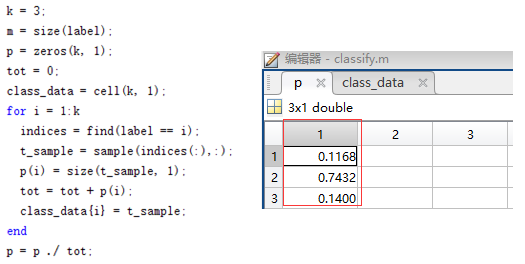
\includegraphics[width=.8\linewidth]{portion}
	\caption{各个睡眠阶段的比例}
	\label{fig:portion}
\end{figure}

\subsection{进行DTFT变换}

正如前文所述,利用计算机的FFT变换,将原本样本的时域特征变换成基于频域的特征。
在完成FFT变换后,我组绘制出三类样本所分别对应的平均FFT示意图。
进行对图片的观察后,我们得出了一系列可供参考的信息。

\subsubsection{观察频谱分布}

首先观察低频部分(见图~\ref{fig:lowf}):

\begin{figure}[ht]
	\centering
	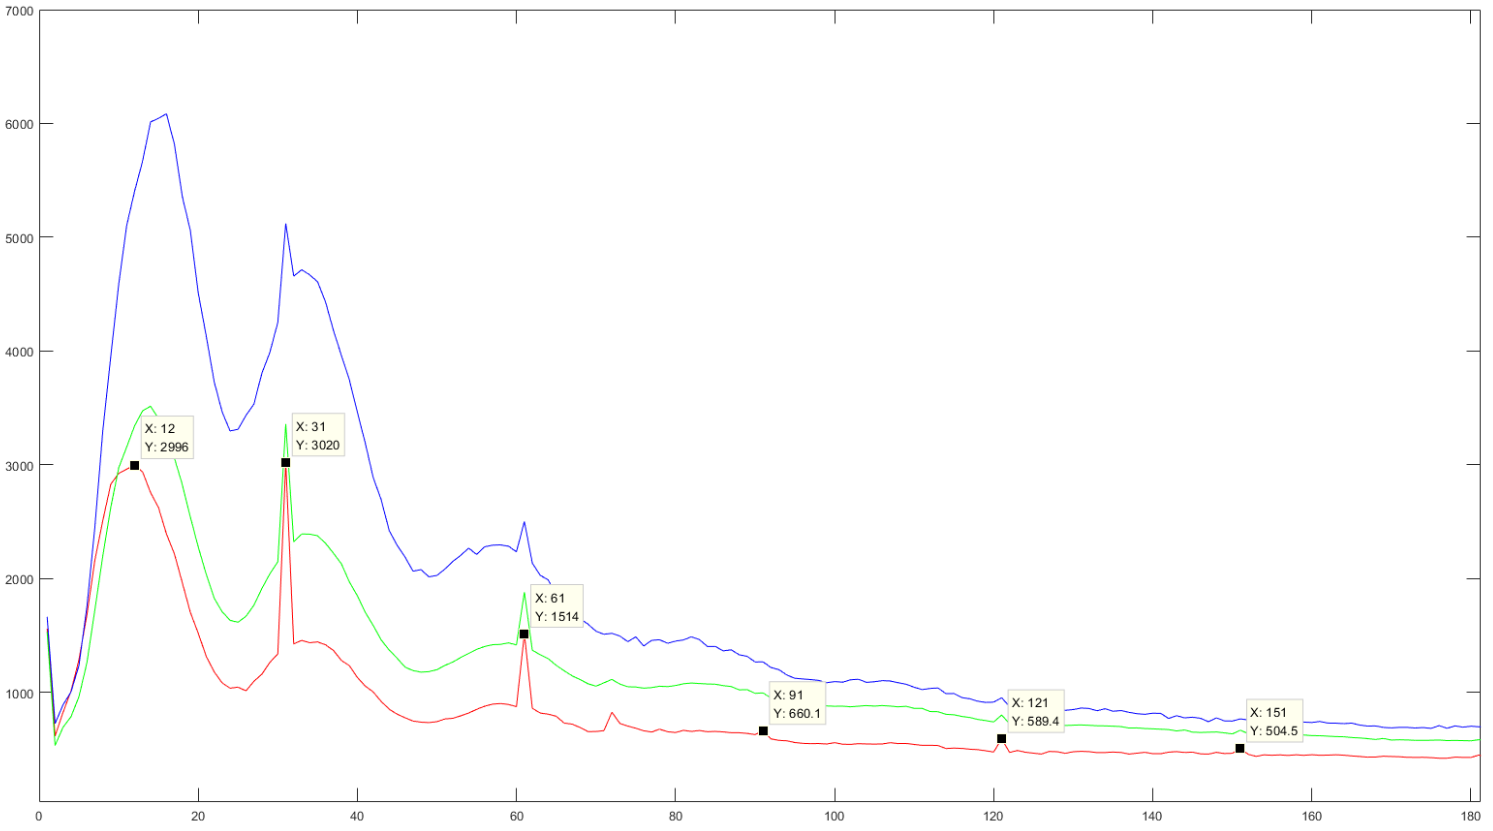
\includegraphics[width=.8\linewidth]{lowf}
	\caption{低频部分频谱分布}
	\label{fig:lowf}
\end{figure}

从上图我们可以清晰地看出在[1, 20]、[25, 40]、[50, 70]这几个频域有三个峰而且不相互重叠,
所以这几个频域能较好地表征原信号。

通过观察还可以发现,每30个频率点会出现一个异常高的尖峰,这个尖峰与其周围频谱分布极其不符,
同时每隔30个频率出现,所以我们考虑这些采样点的成分是原信号中的某种噪声或者异常偏差。
基于以上分析,我们移除这几个异常值后再进行后续处理中。

再观察高频部分(见图~\ref{fig:fivep}):

\begin{figure}[ht]
	\centering
	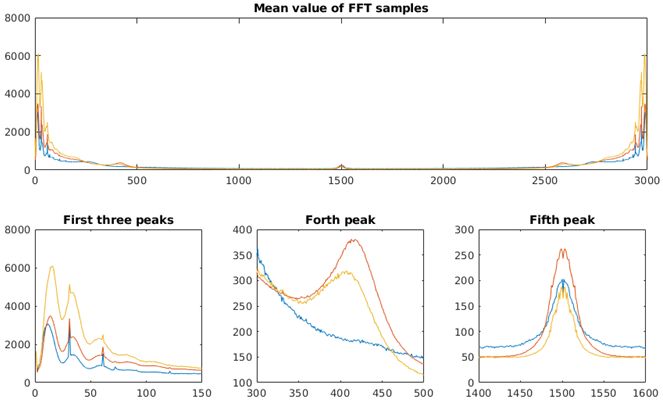
\includegraphics[width=.9\linewidth]{fivep}
	\caption{全频谱分布}
	\label{fig:fivep}
\end{figure}

在[350, 480]、 [1450, 1550]这两个频域还有比较明显的峰。

所以我们最后选取[1, 20]、[25, 40]、[50, 70]、[350, 480]、 [1450, 1550]这五个频段作为特征
进行后续处理。

\subsubsection{消除抖动}

由于单个样本的FFT曲线抖动较为剧烈,所以本文使用中值滤波对频谱分布做平滑处理。
事实上,中值滤波是一种基于排序统计理论的,能有效抑制噪声的非线性信号处理技术。
其原理在于把数字序列中一点的值用该点的一个邻域中各点值的中值代替,
让周围的值接近的真实值,从而消除孤立的噪声点。

\MATLAB 提供了非常便捷的中值滤波接口:\lstinline| medfilt1(fft_sample);|将\\
\lstinline|fft_sample|中每一列的每个值替换为这个值和上下相邻两行值得平均值。

\subsubsection{提取主频}

5.2.1小结介绍了选取频谱中的五个峰,这五个峰包含了原信号中的绝大部分的成分。
进一步观察,每个睡眠阶段在这五个峰的幅值都不尽相同,所以考虑将这五个频域中的最大值选出来,
作为五个特征。

以上所述三个操作的实现如下:

\begin{lstlisting}[language=Matlab]
function [res] = process(sample)
	ff_sample = abs(fft(sample, 3000, 2));
	% 5 peak: [1, 20], [25, 40], [50, 70], [350, 480], [1450, 1550]
	p1 = 1:20;
	p2 = [25:30, 32:40];
	p3 = [50:60, 62:70];
	p4 = 350:480;
	p5 = 1450:1550;
	sam = medfilt1(fft_sample')';	% 中值滤波
	mx1 = max(sam(:, p1), [], 2);
	mx2 = max(sam(:, p2), [], 2);
	mx3 = max(sam(:, p3), [], 2);
	mx4 = max(sam(:, p4), [], 2);
	mx5 = max(sam(:, p5), [], 2);
	comp = [1:20, [25:30, 32:40], [50:60, 62:70], 350:480, 1450:1550];
	fft_sample = fft_sample(:,comp);
	res = [fft_sample, mx1, mx2, mx3, mx4, mx5];
end
\end{lstlisting}

\subsection{数据正则化}

本实验在进行主成分分析前,对各个特征做标准正态化(normalize)。
因为PCA算法选择每个分量的时候,都尽量使得投影其上的数据尽量分散,
所以如果有个维度的数据过于分散,PCA在选取投影向量的时候就会偏向于选取该特征所在的分量,
从而丢失了较多其他维度的信息。事实上,我们得到的样本数据都是多个维度的,
即一个样本是用多个特征来表征的。但是,这些特征的量纲和数值的量级不一定一样。
如果直接使用原始的数据值,那么他们对预测目标的影响程度将是不一样的。
而通过标准化处理,可以使得不同的特征具有相同的尺度。这样,在使用梯度下降法学习参数的时候,
不同特征对参数的影响程度就一样了。

为了解决上述问题,我组将特征数据进行均值为0、方差为1的正态分布转换(见图~\ref{fig:norm})。

\begin{figure}[ht]
	\centering
	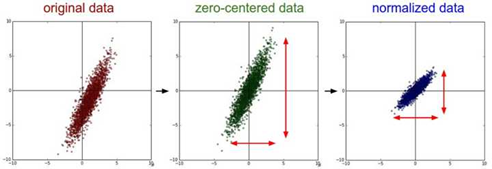
\includegraphics[width=.8\linewidth]{norm}
	\caption{数据正则化}
	\label{fig:norm}
\end{figure}

\subsection{PCA处理}

进过之前提取主要主要频率成分的操作,考虑进一步降低特征的维度。
利用PCA对正则化后的fft样本进行降维,经过试验,当选取6个主成分的时候,
已经能保留原数据中80\%以上的分布信息,训练结果也达到最好。

\begin{lstlisting}[language=Matlab]
[vec, pca_param] = pca_vec(fft_sample, 6, 1);
norm_sample = pca_trans(process(sample), vec, pca_param);
norm_tsample = pca_trans(process(tsample), vec, pca_param);
\end{lstlisting}

\subsection{移出异常值}

经过观察,特征值得分布近似符合正态分布,于是考虑将偏离均值3个标准差以上的数据
视作异常数据剔除。

\begin{lstlisting}[language=Matlab]
function [fil_sam, fil_lab, param] = rm_outlier(sample, label, param)
	m = size(sample, 1);
	idx = [];
	for i=1:m
		if sum(abs(sample(i,:) - param.mu) > 3 * param.std) == 0
			idx = [idx i];
		end
	end
	fil_sam = sample(idx,:);
	fil_lab = label(idx,:);
end
\end{lstlisting}

\subsection{数据归一化处理}

本实验为采用数据归一化,我组认为在神经网络训练中也有必要进行数据归一。

数据归一化,就是将数据映射到[0,1]或[-1,1]区间或更小的区间,比如(0.1,0.9),需要将训练和测试数据进行归一化的原因如下:

\begin{enumerate}
	\item 输入数据的单位不一样,有些数据的范围可能特别大,导致的结果是神经网络收敛慢、训练时间长。
	\item 数据范围大的输入在模式分类中的作用可能会偏大,而数据范围小的输入作用就可能会偏小。
	\item 由于神经网络输出层的激活函数的值域是有限制的,因此需要将网络训练的目标数据映射到激活函数的值域。
	例如神经网络的输出层若采用S形激活函数,由于S形函数的值域限制在(0,1),也就是说神经网络的输出只能限制在(0,1),
	所以训练数据的输出就要归一化到[0,1]区间。
	\item S形激活函数在(0,1)区间以外区域很平缓,区分度太小。例如S形函数$f(X)$在参数a=1时,$f(100)$与$f(5)$只相差0.0067。
\end{enumerate}

\subsection{创建神经网络进行训练}

\begin{figure}[ht]
	\centering
	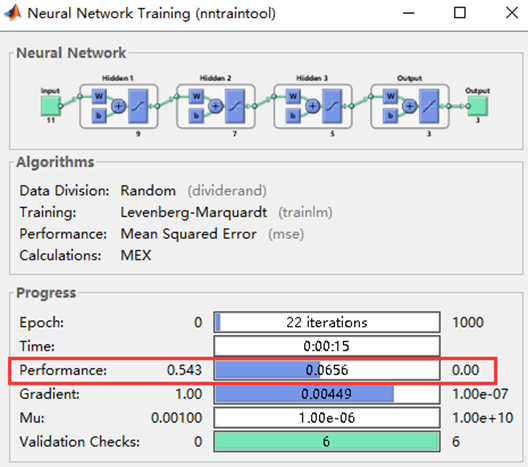
\includegraphics[width=.8\linewidth]{nnet}
	\caption{神经网络训练结果}
	\label{fig:nnet}
\end{figure}

本实验采用feedforwardnet创建训练网络,该网络结构为五层网络,出去输入层和输出层,
还有中间三层隐层。从下图中可以看出输入层为11维,即所选出的6维主成分及5维傅里叶变换主频。
中间层分别为9维、7维、5维,通过原本11维的特征,依次递减,既能有效地保持数据特征,又能逐渐收敛,得到结果输出。